
Extracting knowledge from raw data is an everyday activity for many researchers
and practitioners, in very diverse domains --- from finance to physics.
This is usually referred to as \gls{KDD} because ``knowledge'' is the product of this
process \parencite{Piatetsky-Shapiro1991,Fayyad1996a}. \emph{Data Mining} is sometimes
used as a synonym, or as an integral part \parencite{Fayyad1996a,Reinartz1999}, which is
the preferred interpretation for this work.

\begin{figure}[htbp]
    \centering
    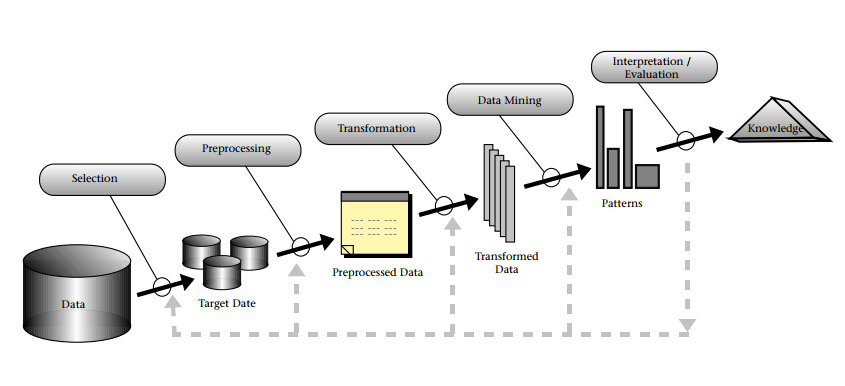
\includegraphics[width=\linewidth]{images/1_introduction/kdd.jpg}
    \caption{\glsfmtfull{KDD}}
    \label{fig:kdd}
\end{figure}

The \gls{CRISPDM}\cite{Shearer2000} proposes a model for the data mining step,
composed of six phases shown in figure \ref{fig:crispdm}:

\begin{description}
    \item[Business Understanding] Definition of the requirements and objectives of a data mining project
        from the business (or domain) perspective.
    \item[Data Understanding] Familiarization with the data collection. Domain knowledge
        is needed to understand the data, but the original project can be refined as the data is best understood.
    \item[Data Preparation] Attribute selection, cleaning, imputation, \ldots are applied over the raw data.
    \item[Modeling] Various modeling techniques are implemented so the questions posed at the first phase
        can be answered.
    \item[Evaluation] Of the proposed models, assessing the quality and suitability of the results.
    \item[Deployment] Or the application of the gained knowledge. This phase can range from integrating
    the chosen models into a system to ``simply'' redacting a report.
\end{description}

\begin{figure}[htbp]
    \centering
    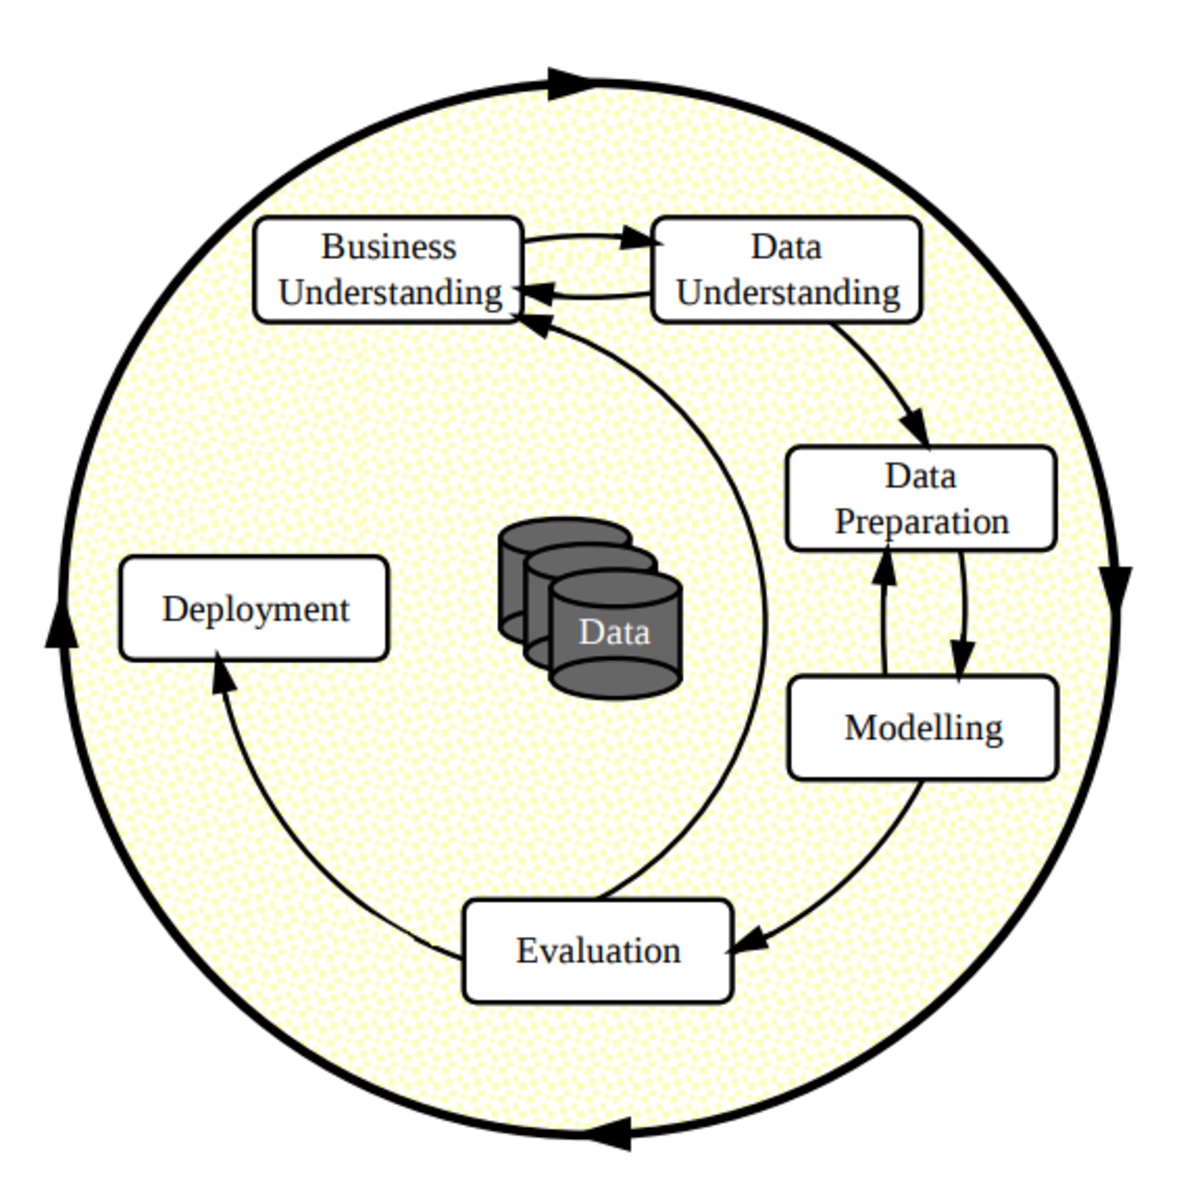
\includegraphics[width=0.8\linewidth]{images/1_introduction/crisp-dm.pdf}
    \caption{\glsfmtfull{CRISPDM}}
    \label{fig:crispdm}
\end{figure}

In this thesis, I will focus on the \textbf{Data Understanding} phase, where the user
explores the data interactively, gaining insight and generating hypotheses during the process \cite{Geer2014}.

When starting the initial analysis, the data may be in a \emph{raw} format: unprocessed files not
optimized for access. Even worse, the design may be inconsistent or poorly documented, and files may
originate from different sources. These factors combined difficult the task of the data scientist:

\begin{itemize}
    \item Ingestion into a ``proper'' database introduces latency. Since the data is not well
        understood, any early design decision will soon become obsolete~\cite{Kersten2011}.
        Techniques for \emph{in situ}~\cite{Idreos2011} exploration try to overcome this difficulty
        by allowing direct examination of the data files performantly.
    \item The data may be split into multiple files~\cite{Baud2012}, and these files may not
        follow the same schema~\cite{Alawini2014}. Data profiling and schema matching tools
        can be helpful for this type of problems.
\end{itemize}

\section{Objectives}

% Support users unknown files main one
% State of the art
% Sample use case: SDSS
% From SDSS queries, most are about describing the model itself
% Multiple files not covered
% Therefore, helping users query without telling them how they might
% seems ignoring one step
% Then the work on equally distributes
% Use plan and reports

Given the problem stated above, the objectives of this thesis are:

\begin{enumerate}
    \item Find and evaluate existing techniques that could help users to understand the data files
        \emph{in situ}.
    \item Identify gaps on the tooling.
    \item Propose improvements or new solutions that could fill those gaps.
    \label{enum:objectives}
\end{enumerate}

\section{Structure of this document}

First, chapter~\ref{chapter:methodology} describes the methodology followed for the
research presented in this thesis. Chapter~\ref{chapter:literature_review} contains
a systematic literature mapping of the \emph{in-situ} processing of scientific data.
Then, chapter~\ref{chapter:diverse} identifies gaps on the literature when it comes
to the exploration of diverse numerical datasets.
Chapter~\ref{chapter:presq} describes an algorithm
suitable for schema matching tailored for scientific data. Chapter~\ref{chapter:som}
outlines a statistical test based on \glspl{SOM}, which can bridge the gap
between schema matching and \emph{in situ} access. Finally, chapter~\ref{chapter:conclusions}
summarizes the findings of this thesis and proposes potential future lines of work.
